% ==========================================================================
%
%  ASCEM: Developers' Guide (Mathematical Modeling Requirements)
%
% ==========================================================================

% --------------------------------------------------------------------------
%  Options for typesetting:
% --------------------------------
% 
%    final     - no watermark
%    draft     - draft watermark
%    sidenotes - adjusts margins and enables the todonotes package
%
%  For example, draft watermark with sidenotes is written
%
%  \documentclass[draft,sidenotes]{guides}
%
% --------------------------------

%\documentclass[sidenotes]{../tex/latex/ascem/guides}
\documentclass[dvipsnames]{../tex/latex/ascem/guides}

% ---------------------
% Amanzi TeX:
% ---------------------

\newcommand{\AmanziTeXInputs}{..}

% ---------------------
%  ASCEM Theme:
% ---------------------

\usepackage{\AmanziTeXInputs/tex/latex/ascem/ASCEM_doc_theme}

% --------------------------------
%  Layout, fonts, macros etc. 
% -------------------------------- 

\usepackage{local}

% ==========================================================================

\begin{document}

% -------------------------------------------
% Title/Cover Page
% -------------------------------------------
%
% =========================================================================
% -------------------------------------------------------------------------
% ASCEM Cover Page:  Process Models
% -------------------------------------------
%
%  Based on the ASCEM Dcoument template the cover package expects
%  the following variables:
%  
%  \DocTitle   - 24pt Font, up to two lines, ~ 6 in. wide.
%  \DocRev     - ASCEM-HPC-YY-nn-rr, where YY-nn-rr are assigned by DOE.
%  \DocDate    - typically today, could be hard wired if necessary.
%  \DocAuthors - Use tabular (up to 4 columns). 
%
% --------------------------------------------------------------------------

\LogoPath{\AmanziTeXInputs/logos}

\DocTitle{%
  Amanzi Theory Guide, \\[10pt]
  \emph{Mathematical Modeling Requirements}
}

\DocRev{AMANZI-SRD-Revision 1}
\DocDate{\today}

\DocAuthors{%
  \begin{tabular}{llll}
  V. Gyrya, LANL &
  K. Lipnikov, LANL & 
  D. Moulton, LANL &
  S. Molins, LBNL  
  \\[-3pt]
  C. Steefel, LBNL &
  &
  & 
  \end{tabular}
}



\ASCEMcover

\begin{textblock}{12}(0, 1)
This version of the document was based on 
\emph{``Mathematical Formulation Requirements and Specification for the Process Models''},
version ASCEM-HPC-2011-01-0c.\\

\begin{tabular}{llll}
  C. Steefel, LBNL &
  P. Lichtner, LANL & 
  J. Bell, LBNL &
  G. Zyvoloski, LANL
  \\[-3pt]
  D. Moulton, LANL & 
  T. Woley, LLNL &
  G. Moridis, LBNL &
  B. Andre, LBNL 
  \\[-3pt]
  G. Pau, LBNL &
  D. Bacon, PNNL &
  S. Yabusaki &
  L. Zheng, LBNL
  \\[-3pt]
  K. Lipnikov, LANL &
  N. Spycher, LBNL &
  E. Sonnenthal, LBNL &
  J. Davis, LBNL
  \\[-3pt]
  J. Meza, LBNL & & & \\
\end{tabular}
\end{textblock}

\ASCEMdisclaimer

% =========================================================================


% -------------------------------------------
% Table of Contents
% -------------------------------------------
%
\clearpage
\setcounter{tocdepth}{2}
\tableofcontents

% -------------------------------------------
% List of Tables and Figures
% -------------------------------------------

\clearpage
\listoftables
\listoffigures

% -------------------------------------------
% Todo Notes list
% -------------------------------------------

\ifthenelse{\boolean{sidenotes}}{%
  \clearpage
  \listoftodos[ToDo List]
}%else
{}

% -------------------------------------------
% Content: 
% -------------------------------------------

% Sections:

\clearpage
% -------------------------------------------------------------------------
%  This is a good place to outline key objectives of this section.
% -------------------------------------------------------------------------

\section{Introduction}

\subsection{Purpose and Scope of this Document}
This document provides description of Amanzi libraries, summarizes design concepts,
provides step-by-step instructions and detailed comments for solving an abstract PDE,
provides essentials on creation of unit tests and web-pages for the user guide.

The intended audience includes (a) new developers of Amanzi and (b) software developers
who wants to use general purpose C++ Amanzi libraries in their work. 

This document is not designed for the end-users who want to use Amanzi as the 
subsurface simulator.


\subsection{Organization and Layout of this Document}

To be written last.








\clearpage
% -------------------------------------------------------------------------
%  This is a good place to outline key high-level design principled
% -------------------------------------------------------------------------

\section{Design of Amanzi}

In short, the guiding  principles described below are related to code readability,
modularity, and extensibility.
We facilitate community code development and code review, we follow closely, but not exactly, 
the Google C++ coding style, see 
\begin{center}
{\tt https://google.github.io/styleguide/cppguide.html}
\end{center}

for more detail.
In this section, we describe high-level principles and elaborate some of them 
in the subsequent section.
We use different fonts to distinguish between a {\tt Class} name, its {\it Methods()}, 
and its {\it variables}. 
Global {\rm CONSTANTS} are capitalized.

\underline{Disclaimer}. Amanzi's initial code implementation of new models 
and algorithms does not always comply with the formulated design principles, but 
it is getting there with each code re-factory.


%%%%%%%%%%%%%%%%%%%%%%%%%%%%%%%%%%%%%%%%%%%%%%%%%%%%%%%%%%%%%%%%%%%%%%
\subsection{State}
State is a simple data manager. 
It allows process kernels (PK) to require, read, and write various variables (such as physical fields).
It guarantees data protection by providing both const and non-const data pointers for variables.
It provides some initialization capability -- this is where all independent variables can be 
initialized -- since independent variables are typically owned by the state, not by a process kernel.
A few initialization tools are supported: a space-time function, initialization from an Exodus file 
and initialization from an HDF5 file.



%%%%%%%%%%%%%%%%%%%%%%%%%%%%%%%%%%%%%%%%%%%%%%%%%%%%%%%%%%%%%%%%%%%%%%
\subsection{PK and MPC PK}
PK stands for the Process Kernel.
MPC stands for the Multi-Process Coupler.
Each PK and MPC PK does little actual numerical work.
Instead, PK administrates discretization schemes, time integrators, and solvers. 
Each PK may represent a single equation (e.g. the Poisson equation for the Darcy flow) 
or system of strongly connected equations (e.g. the Navier-Stokes flow).

An MPC PK couples multiple physical processes which have their respected PKs.
One example is the Darcy flow and dispersive transport of chemical components.
An MPC PK may often be fully automated with no knowledge of the underlying PKs.
Since an MPC PK has the same interface as a PK, it is also a process kernel which
allows us to build a hierarchy of physical models with various degree of coupling
ranging from a weak coupling to an iterative coupling to a strong coupling.

Much of the work in a PK is delegated to field evaluators, which implement various 
physical and mathematical models, such as the equations of state, or boundary conditions, 
or mesh deformation. 
For these reasons, it is appropriate to call them variable evaluators.
The available variable evaluators are classified as follows:

\begin{enumerate}
\item Independent variable evaluators are the user-provided functions of spatial and temporal coordinates
      and has no dependencies.
      They could be used to compute (analytic or tabulated) boundary conditions, source terms, and initial conditions. 
\item Primary variable evaluators are related to the fields solved for within a PK.
      Examples are pressure and temperature fields.
      Typically these evaluators are used internally to track change in fields state and inform the 
      dependency tree about this.
\item Secondary variable evaluators are derived either from primary variable evaluators or other secondary variables. 
      There are two types of the secondary variable evaluators used to evaluate either a single or multiple variables.
      A model for a secondary variable can be anything from a constitutive relation to a discrete operator
      (apply a divergence operator to a velocity given a mesh and discretization) 
      to a summation operator (add the divergence of Darcy fluxes to a source term to determine the mass balance).
      Quite often, the secondary field/variable evaluators are created by high-level PKs during the setup phase 
      and inserted automatically in the list of evaluators. 
\end{enumerate}

The evaluator is much like a functor or function; it stores no actual data, only meta-data and 
a few parameters or constants.
It accesses data using a data manager, which controls access for both read-only and read/write modes. 

All evaluators are stored in a dependency graph, which is a directed, acyclic graph (DAG) 
describing the functional relationship of each variable in the state. 
End nodes in the dependency graph are either independent variables or primary variables. 
All other nodes in the graph are secondary variables.

The combination of a data manager and a dependency graph enables dynamic definition of each variable's model 
and data, and splits complex equations into manageable chunks. 
It also allows lazy evaluation, where nodes in the graph are updated (re-calculated) only if their dependencies
have changed, resulting in a managed, automated evaluation process with fewer bugs and inefficiencies.
For more details, we refer to \cite{coon2016managing}.
A developer may easily modify behavior of evaluators by overriding virtual member functions. 
The example below shows implementation of one function in an abstract product evaluator of type 
$\Pi_{i=1}^N f_i^{p_i}$ where $p_i$ is either 1 or -1.

\begin{lstlisting}[language=C++]
void ProductEvaluator::EvaluateField_(
    const Teuchos::Ptr<State>& S,
    const Teuchos::Ptr<CompositeVector>& result)
{
  auto& result_c = *result->ViewComponent("cell");
  int ncells = result_c.MyLength();

  int n(0);
  result_c.PutScalar(1.0);
  for (auto it = dependencies_.begin(); it != dependencies_.end(); ++it) {
    const auto& field = *S->GetFieldData(*it)->ViewComponent("cell");
    if (powers_[n] == 1)
      for (int c = 0; c != ncells; ++c) result_c[0][c] *= field[0][c];
    else if (powers_[n] == -1)
      for (int c = 0; c != ncells; ++c) result_c[0][c] /= field[0][c];
    n++;
  }
}
\end{lstlisting}



%%%%%%%%%%%%%%%%%%%%%%%%%%%%%%%%%%%%%%%%%%%%%%%%%%%%%%%%%%%%%%%%%%%%%%
\subsection{CompositeVector}
Class {\tt CompositeVector} is an implementation of an improved
{\tt Epetra\_MultiVector} (from Trilinos suite of packages) which spans multiple components and knows how to
communicate itself.
A composite vector is a collection of vectors defined on a common mesh and
communicator. 
Each vector, or component, has a name (typically, a mesh entity)
and a number of degrees of freedom.  
This meta data is stored in class {\tt CompositeVectorSpace}.
For instance, the field {\it total\_component\_concentration} is the cell-centered field with 
as many degrees of freedom as there exist chemical components.

Ghost cell updates are managed by the class {\tt CompositeVector}. 
Design of the parallel communication strategy is driven by two observations:
\begin{itemize}
\item The need for updated ghost cell information is typically known by the
      user just prior to being used, not just after the master values are
      updated.
\item Occasionally multiple functions need ghost values, but no changes to
      owned data have been made between these functions.  However, it is not
      always possible for the second call to know, for certain, that the first
      call did the communication.  Versatility means many code paths may be
      followed.
\end{itemize}


\subsubsection{Parallel communications}
To avoid unnecessary parallel communication the following algorithms were implemented
but are not active now.
This may change in the future.

Each time the vector values are changed, an internal flag is marked to
record that the ghost values are stale.
Each time ghost cells are needed, that flag is checked and communication
is done, if needed.
Keeping this flag correct is therefore critical. 
To do this, access to vectors must follow the rigid pattern.
The following modifications tag the flag:

\begin{enumerate}
\item Any of the usual {\it PutScalar()}, {\it Apply()}, etc methods.
\item Non-const calls of {\it ViewComponent()}.
\item Call of {\it GatherMasterToGhosted()} and {\it ChangedValues()}.
\item {\it Scatter()} called in a non-{\rm INSERT} mode.
\end{enumerate}

There exist known ways to break this paradigm. 
One is to store a non-const pointer to the underlying {\tt Epetra\_MultiVector}.
The fix is simple as this: \underline{never} store a pointer to the underlying data, 
just keep pointers to the composite vector itself.

The other one is when one grabs a non-const pointer, calls {\it Scatter()}, then 
changes the values of the local data.  
This is the nasty one, because it is both subtle and reasonable usage.
When you access a non-const pointer, the data is flagged as changed.
Then you call {\it Scatter()} and the data is flagged as unchanged.
Then you change the data from your old non-const pointer, so that the data is changed, but not flagged.
The first fix is to always call {\it ViewComponent()} after {\it Scatter()} and before changing values.
Another way to protect yourself is to put non-const references in their own scope.
For instance, the following practice is encourage:
\begin{lstlisting}[language=C++]
CompositeVector my_cv;
{ // unnamed scope for my_vec
  Epetra_MultiVector& my_vec = *my_cv.ViewComponent("cell", false);
  my_vec[0][0] = 12;
} // close scope of my_vec

my_cv.ScatterMasterToGhosted()

// Reference to my_vec is now gone, so we cannot use it and screw things up!

{ // unnamed scope for my_vec
  // This is now safe!
  Epetra_MultiVector& my_vec = *my_cv.ViewComponent("cell", true);
  my_vec[0][0] = my_vec[0][ghost_index] + ...
} // close scope of my_vec
\end{lstlisting}

The final way to break the parallel machinery is to use {\it const\_cast()} and 
then change the values.
Const-correctness is your friend. Keep your PKs const-correct, and you will never have this problem.

Note that the non-{\rm INSERT} modes of scatter are never skipped because of the flag state, 
and the flag is always tagged as changed.  
This is because subsequent calls with different modes would break the code.


%%%%%%%%%%%%%%%%%%%%%%%%%%%%%%%%%%%%%%%%%%%%%%%%%%%%%%%%%%%%%%%%%%%%%%
\subsection{TreeVector}
The class {\tt TreeVector} implements a nested, hierarchical data structure 
that mimics that for PK hierarchies.
It is an extendable collection of composite vectors.
This vector allows each physical PK to use composite vector to store 
their solution, and allows MPCs to push back vectors in a tree format.

This class provides the standard vector interface (extended ring algebra) and 
may be used with time integrators and nonlinear solvers.


%%%%%%%%%%%%%%%%%%%%%%%%%%%%%%%%%%%%%%%%%%%%%%%%%%%%%%%%%%%%%%%%%%%%%%
\subsection{Linear operators}
The idea behind the design of Amanzi operators is to separate three 
functionalities that are frequently placed in a single class in other
C++ packages.

\begin{enumerate}
\item Containers of local matrices (classes prefixed with {\tt Op}) and 
      data layout {\it schemas}.

\item Linear operators and elemental operations with them: assembly of a global 
      matrix (e.g. Jacobian), matrix-vector product, inversion, and calculation of the Schur complement.

\item Discrete PDEs: populate values in local matrices, add nonlinear 
coefficients, create specialized preconditioners, and impose special
boundary conditions. 
\end{enumerate}


\subsubsection{Op}
Class {\tt Op\_*} is a container of local matrices.
A series of such classes (e.g. {\tt Op\_Cell\_FaceCell} and {\tt Op\_Cell\_Schema}) handle data layout. 
The second word in the class name indicates the container size (the number of mesh cells here).
The third word specifies location of degrees of freedom: in cells and on faces in the first example;
specified by a complex schema in the second example.
These are really just structs of vectors of
dense matrices of doubles, and simply provide a type.
They are derived from the virtual class {\tt Op}.

A key concept of an {\tt Op} is the schema. 
The old design of the schema includes one enum representing the dofs associated
with the Operator's domain and range, and one enum for the contained size. 
This is a major limitation for implementing complex discretization schemes.
Also a single schema implies that the domain and range of the operator are the same.
The new design (which is backward compatible) includes two schemas that are also more 
detailed. A the first enum is replaced with the list of enums to represent various 
possible collections of degrees of freedom including non-standard degrees of freedom 
as as derivatives and moments.
Additional list specifies multiplicity of these degrees of freedom.
The second enum in the new schema specifies (as before) the geometric entity over which the local 
matrices are assembled.

Existence of two (simple and complex) schemas provides some flexibility for code development.
For instance, a developed could create surface matrices, and then assemble them into a 
subsurface matrix by introducing a new {\tt Op} class (for surface discretization) with a simple schema.
Alternatively, it could be done using the class {\tt Op\_Cell\_Schema} with a complex schema. 

The general schema makes it trivial to assemble a global matrix (e.g. in a coupled flow-energy system)
from sub-block operators.
Finally, the new schema supports rectangular matrices which is useful for saddle-point 
type systems.

{\tt Op\_*} works via a visitor pattern.
Matrix assembly, {\it Apply()}, application of boundary conditions, and symbolic assembly 
are implemented by the virtual class {\tt Operator} calling a dispatch to the 
virtual class {\tt Op}, which then dispatches back to the derived class {\tt Operator\_*} so that
type information of both the {\tt Operator\_*} (i.e. global matrix info) and 
the {\tt Op\_*} (i.e. local matrix info) are known.

A container of local matrices (i.e. instantiation of a {\tt Op\_*}) 
can be shared by multiple {\tt Operator\_*}. 
Sharing is indicated by the variable {\it ops\_properties}. 
In combination with {\it CopyShadowToMaster()} and {\it Rescale()},
a developer has a room for a variety of optimized implementations.
The key parameters have prefix {\rm OPERATOR\_PROPERTY} and described in file {\it Operators\_Defs.hh}.


\subsubsection{Operator}
An operator represents a map from linear space $X$ to linear space $Y$.
Typically, this map is a linear map; however, it can be used also to calculate
a nonlinear residual. 
The spaces $X$ and $Y$ are coded using class {\tt CompositeVectorSpace}.
A few concrete maps $X \to Y$ are already implemented in the code.

Typically the forward operator is applied using only local Ops.
The inverse operator typically requires assembling a matrix, which 
may represent the entire operator or may be only its Schur complement.

The class {\tt Operator} performs actions summarized in the second bullet above. 
Amanzi has a few derived classes such as {\tt Operator\_Cell}, {\tt Operator\_Node}, 
{\tt Operator\_FaceCellSff}, where the suffix {\tt \_X} indicates the specific map,
see class {{\tt Operator\_Schema} for a general map.
These classes are derived from the virtual class {\tt Operator} which stores a
schema and a pointer to a global operator.

Concrete maps use the old schema which is an integer variable.
Their are now superseded by the new flexible schema which is a class variable.
Each operator stores a list of containers of local matrices, more precisely 
a list of pointers to the variables of class {\tt Op}.

The only potentially confusing part is the use of the visitor pattern (i.e. double 
dispatch in this case) to resolve all types.  
For instance to assemble a matrix, we may use the following pseudocode

\begin{lstlisting}[language=C++]
// Operator
AssembleMatrix(Matrix A) {
  for each op {
    op->AssembleMatrix(this, Matrix A);
  }
}

virtual AssembleMatrixOp(Op_Cell_FaceCell& op) { 
  // throw error, not implemented
}

// Op
AssembleMatrix(Operator* global_op, Matrix& A) = 0;

// Op_Cell_FaceCell
AssembleMatrix(Operator* global_op, Matrix& A) {
  global_op->AssembleMatrixOp(*this, A);
}

// Operator_FaceCell
AssembleMatrixOp(Op_Cell_FaceCell& op, Matrix& A) {
  // This method now know both local schema and the matrix's dofs, 
  // and assembles the face+cell local matrices into the matrix.
}
\end{lstlisting}

The reason for the double dispatch is to get the types specifically
without a ton of statements like this one "if (schema == schema1) 
\{ assemble one way \} else \{ assemble another way\}".


\subsubsection{PDE}
A "discrete" PDE consists of (a) a single global operator, (2) an 
optional global assembled matrix, and (3) an un-ordered additive collection of 
lower-rank (or equal rank) local operators, hereafter called {\it ops}. 
During its construction, a PDE can grow by assimilating more {\it ops}. 
The global operator knows how (a) to perform the matrix-vector product, 
the corresponding function is called {\it Apply()}, and (b) to assemble {\it ops} into a global matrix.
Each {\tt PDE\_*} class knows how to apply boundary conditions and to create a preconditioner.

The classes {\tt PDE\_Diffusion}, {\tt PDE\_Advection},{\tt PDE\_Accumulation}, etc create 
operators of the specified type (for instance 
{\tt Operator\_FaceCell} or {\tt Operator\_Schema}), populate their values, and
apply boundary conditions.
They are in some sense physics based generalization of operators and may perform complex actions
such as an approximation of Newton correction terms.

A collection of PDEs that store a pointer to the same global operator form an additive PDE.
Application of boundary conditions is done independently by each PDE in this collection.
The result is gathered into a single right-hand side vector.


Discretization of a simple 
PDE (i.e. diffusion) is not done directly. 
Instead, a helper class that contains methods for creating and populating 
the {\it ops} within the {\tt Operator} is used. 
The helper class can be used to discretize a simple PDE, such as the diffusion equation.
A more complex PDE, such as the advection-diffusion equation, can be discretized 
by creating two "discrete" PDEs for diffusion and advection processes.


%%%%%%%%%%%%%%%%%%%%%%%%%%%%%%%%%%%%%%%%%%%%%%%%%%%%%%%%%%%%%%%%%%%%%%
\subsection{TreeOperator}
Class {\tt TreeOperator} is the block analogue of linear operators and 
provides a linear operator acting on a {\tt TreeVectorSpace}. 
In short, it is a matrix of operators.
Currently this structure is used for things like multiphase flows, 
thermal Richards, coupled matrix-fracture flow and transport, etc.


%%%%%%%%%%%%%%%%%%%%%%%%%%%%%%%%%%%%%%%%%%%%%%%%%%%%%%%%%%%%%%%%%%%%%%
\subsection{Linear solvers}
Native and third-party solvers are handled through a single factory and 
the uniform interface.
Direct and iterative solvers from Trilinos is a part of this factory.
Native re-implementation of some iterative solvers supplied by Trilinos
is due to lack of capabilities needed for subsurface solvers.
One example is the neccisety to perform at least one iteration even when
a norm of the linear residual is below the requested tolerance.


%%%%%%%%%%%%%%%%%%%%%%%%%%%%%%%%%%%%%%%%%%%%%%%%%%%%%%%%%%%%%%%%%%%%%%
\subsection{Nonlinear solvers}
A factory of nonlinear solvers includes sever solvers ranging from
the Newton method to inexact Newton methods to continuation methods.
The solvers are templated on classes {\tt Vector} and {\tt VectorSpace}.

The nonlinear Krylov accelerator solvers \cite{carlson1998design} implements
inexact Newton's method, where the correction 
equation of Newton's method is only approximately solved because the 
Jacobian matrix is approximated and/or the linear system is not solved exactly.  
Placed in the iteration loop, this black-box accelerator listens to the sequence
of inexact corrections and replaces them with accelerated corrections;
the resulting method is a type of accelerated inexact Newton method.
Note that an inexact Newton iteration is merely a standard fixed point iteration for
a preconditioned system, and so this accelerator is more generally
applicable to fixed point iterations.




\clearpage
\section{Selected Amanzi libraries}

This section describes Amanzi libraries, their limitations and possible 
ways to extend.

\subsection{WhetStone}
This is a low-level library that implements primarily local matrices for 
various discretizations schemes. 
Conceptual dosing of this part of the library is presented in Fig.~\ref{fig:whetstone}.
Classes derived from class {\tt MFD3D} cover a huge spectrum of elliptic
operators.

Additional functionality included in this library supports
\begin{enumerate}
\item the ring algebra of scalar, vector and matrix polynomials;
\item quadrature rules on simplices;
\item numerical integration algorithms based on the Euler homogeneous theorem;
\item coordinate transformations including parameterization of mesh faces and edges.
\end{enumerate}

A few  comments on the design principles. 
Polynomial coefficients are represented by a linear array. 
An polynomial iterator class allow us to access information about monomial terms of 
a given polynomial in a for-type loop:
\begin{lstlisting}
Polynomial poly(3, 2);
for (auto it = poly.begin(); it < poly.end(); ++it) {
  int i = it.PolynomialPosition();
  int k = it.MonomialSetOrder();
  const int* idx = it.multi_index();
  double ci = poly(i);
}
\end{lstlisting}
Each step of this loop extracts information about monomial $c_i \,x^{idx_0} y^{idx_1} z^{idx_2}$
of order $k= idx_0 + idx_1 + idx_2$ in a quadratic polynomial.

Quadrature rules on simplexes have positive weights for stability of numerical schemes. 
Integration formulas based on Euler's homogeneous theorem can be used for integrating
polynomials over polytopal cells.
To integrate polynomial and non-polynomial functions using a single interface a simple
base class {\tt WhetStoneFunction} is used.

Coordinate transformation allows us to treat a 3D mesh face as a 2D polygon.
This is used in (a) hierarchical construction of high-order virtual element and mimetic 
schemes, and (b) projection of polynomials on a low-dimension manifold and an reserve (non-unique)
lifting operation.

Finally library {\it WhetStone} contains a factory of discretization schemes that could
be extended by including users schemes via simple interface.
Example of such an extension is available in Operator's tests.


\begin{figure}[h!]
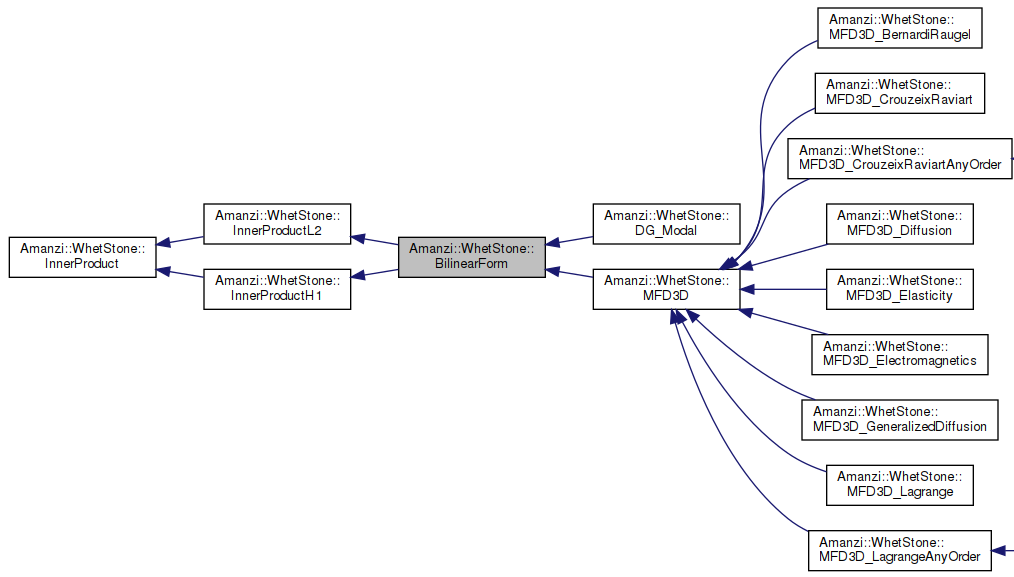
\includegraphics[width=1.0\textwidth]{figs/whetstone.png}
\caption{Partial dependency tree for library WhetStone.\label{fig:whetstone}}
\end{figure}

\clearpage
\subsection{Operators}

\begin{figure}[h!]
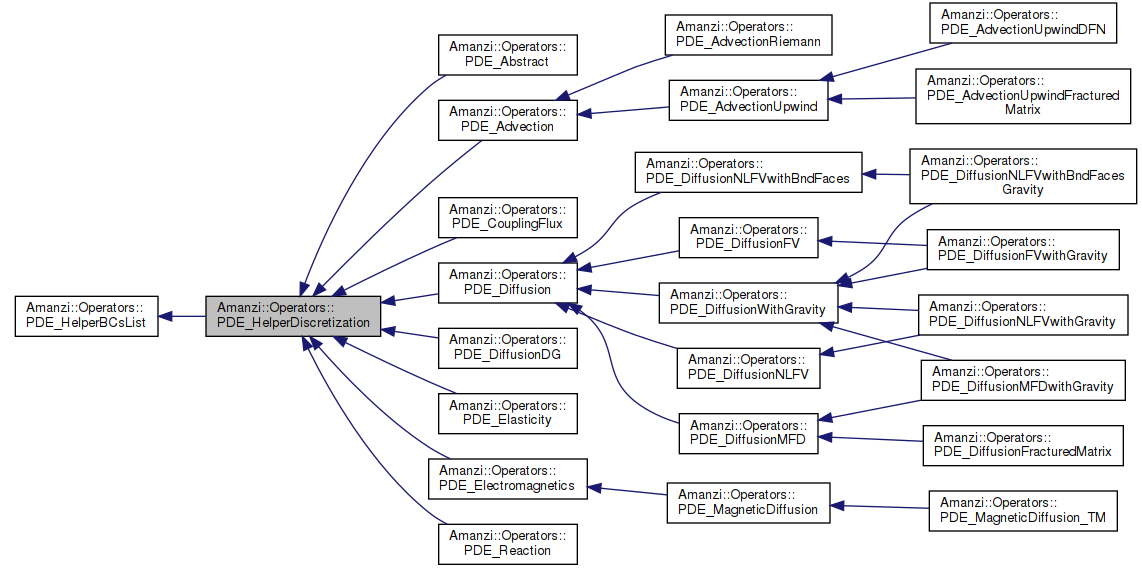
\includegraphics[width=1.0\textwidth]{figs/operators.png}
\caption{Partial dependency tree for library Operators.\label{fig:operators}}
\end{figure}


\subsection{PKs}

Bla-bla-bla



\clearpage
\section{Synthetic example}
The purpose of this section is to shed some light into solving square systems using Amanzi. A square systems are those that can be written as
%
\begin{equation}
\mbox{Find }u\in V:\;\forall v\in V\quad
a(u,v) = f(v).
\end{equation}
The types of problems these systems include well-known differential systems like Poisson, Advection-diffusion, magneto and electro statics. In summary, the process of solving these types of systems is as follows, begin by creating a mesh using the mesh\_factory, then create a class for your PDE type as a derived class from PDE\_HelperDiscretization, this will give access to a container for local matrices and a global operator that assembles these matrices as well as routines for applying Dirichlet-type boundary conditions. Thus, the next step is to populate the entries in the container for mass matrices, then assemble the global system and the right-hand side and apply a linear solver.\\


\subsection{Defining your PDE class}\label{Sec:PDEClass}
The PDE class defined must be a derived class of PDE\_HelperDiscretization, this immediately gives 
new class access to two important varibles, a global operator and a container for local matrices and a series of useful routines to apply boundary conditions, assemble global systems, etc. This all comes with a caviat: you must define a member function called UpdateMatrices which is usually used to populate the local matrices, failure to do so will result in an abstract class with no possibility for instantiation.The header for a class to solve the Poisson equation in second order form will look like
%
\begin{lstlisting}
class PDE_SecondOrderPoisson: public PDE_HelperDiscretization {
 public:
  PDE_SecondOrderPoisson(const Teuchos::RCP<const AmanziMesh::Mesh>& mesh);
  ~PDE_SecondOrderPoisson() {};

  // creation of an operator
  using PDE_HelperDiscretization::UpdateMatrices;
  virtual
  void UpdateMatrices(const Teuchos::Ptr<const CompositeVector>& u,
                      const Teuchos::Ptr<const CompositeVector>& p);
		
  // postprocessing: calculated stress u from displacement p
  virtual
  void UpdateFlux(const Teuchos::Ptr<const CompositeVector>& p,
                  const Teuchos::Ptr<CompositeVector>& u) {};
		
  // these are accessors
  Teuchos::RCP<CompositeVectorSpace> GetCVS() { return cvs_; }

 public:
  Teuchos::RCP<CompositeVectorSpace> cvs_;
};
\end{lstlisting}

%
Notice that in this class we have, additionally, defined a composite vector space as a class variable. Composite vector spaces are factories for composite vectors which is an enhanced epetra multivector. This factory can help us create vectors for our trial or test spaces which in the case of a square system are the same or at least have the same set of degrees of freedom. In what follows we will explain how to define the global operator, we note that this is all done in the constructor of the PDE class.
%
\subsubsection{Populating The Local Matrices and Defining the Global Operator}\label{Sec:LocalMatAndGlobalOp}
%
The first step in populating the local matrices is to define a schema. There should be one schema for the test space and one for the trial space, in the case of square systems the same can be used for both. Schemas define the different aspects of a variable and its discretization. Schemas require two inputs: the base and and an item. The base describes what type of assembly is required for this variable the choices include cells, faces, edges and nodes all part of the AmanziMesh namespace. Selecting, for example, faces as the base will imply that the local matrices are associated with the faces of the mesh. Moreover, item defines the type of degrees of freedom that are used to discretize the variable in question. Items require three inputs: a part of the topology of the mesh like a node or an edge which defines where the degrees of freedom are places, the type of quantity the degree of freedom, whether it is scalar of vector valued and the number of degrees of freedom of this type. For a classic finite element method to solve the Poisson equation the definition of its schema will look something like
%
\begin{lstlisting}
Schema p_schema;
// the assembly should run over the cells thus its base are the cells
p_schema.SetBase(AmanziMesh::CELL);

// the pressure DOFs are cell-based and scalars.
p_schema.AddItem(AmanziMesh::NODE,WhetStone::DOF_Type::SCALAR,1);
p_schema.Finalize(mesh);  // computes the starting position of the dof ids
\end{lstlisting}
%
Feeding the mesh to the schema, as shown in the last step, will create important variables used in the eventual assembly.\\
%
Once the necessary schemas are defined the local operator can be initialized and populated in a fairly straight-forward way. It is a matter of feeding the schemas to the local operator and defining the necessary matrices. For example:
%
\begin{lstlisting}
local_op_ = Teuchos::rcp(new Op_Cell_Schema(p_schema,p_schema,mesh));
//Now we populate the local matrices
for (int c = 0; c < ncells_owned ; c++) {
	Mcell(0,0) = 3, Mcell(0,1) = -1, Mcell(0,2) = -1, Mcell(0,3) = -1;
	Mcell(1,0) = -1, Mcell(1,1) = 3, Mcell(1,2) = -1, Mcell(1,3) = -1;
	Mcell(2,0) = -1, Mcell(2,1) = -1, Mcell(2,2) = 3, Mcell(2,3) = -1;
	Mcell(3,0) = -1, Mcell(3,1) = -1, Mcell(3,2) = -1, Mcell(3,3) = 3;
	local_op_->matrices[c] = Mcell;
}
\end{lstlisting}
%
To finalize we need to define the global operator which requires us to fist define a composite vector space that is consistent with the schema that we defined in the local systems. Thankfully schema has a rotine that does this for us. Thus, initializing the global operator can be done in four lines as follows:
\begin{lstlisting}
cvs_ = Teuchos::rcp( new CompositeVectorSpace 
(cvsFromSchema(p_schema, mesh,false)) );
//The constructor for a global operator requires a 
//parameter list so we will create a dummy one
Teuchos::ParameterList plist = Teuchos::ParameterList();
//This line creates a global operator for the mass matrix
global_op_ = Teuchos::rcp(new Operator_Schema(cvs_, plist, p_schema));
//This line assigns the corresponding container of local matrices.
global_op_->OpPushBack(local_op_);
\end{lstlisting}
%
\subsection{Creating A Mesh}\label{CreatingAMesh}
The class MeshFactory gives the necessary tools to create a mesh. Mesh factory requires some inputs: the MPI communicator and the preferences which provide the specific capability that is used. A default communicator is already defined in Amanzi namespace and the preferences are usually set to MSTK anb STK from the namespace Framework.\\
The meshfactory object can create meshes in several ways depending on the dimensionality (2D or 3D) and the types of cells. A complete routine to build a simple quadrilateral mesh in 2D will look like this: 
%
\begin{lstlisting}
auto comm = Amanzi::getDefaultComm();
MeshFactory meshfactory(comm);
meshfactory.set_preference(Preference({Framework::MSTK, Framework::STK}));
// Generates a structured mesh covering [x0,x1] X [y0,y1] with (nx, ny)
// cells.
//  Teuchos::RCP<Mesh> create(const double x0, const double y0,
//                           const double x1, const double y1,
//                           const int nx, const int ny,
//                           const bool request_faces=true,
//                           const bool request_edges=false);
Teuchos::RCP<const Mesh> mesh = meshfactory.create(-1,-1,1,1,3,3);
\end{lstlisting}
%
The classes MeshFactory and Mesh are a part of MSTK for which documentation is available. 
%
\subsection{Adding boundary conditions}\label{Sec:AddingBoundaryCond}
The class PDE\_HelperDiscretization has some built in features to impose boundary conditions but in order to access them we need to define the object BCs which takes as creation arguments the mesh, where the degrees of freedom will be places and the type of degree of freedom. Moreover, we must also populate the two class variables, the bc\_model which defines what type of boundary condition we want to prescribe and the bc\_value which precise value of such boundary condition. For example,
%
\begin{lstlisting}
//The BCs are placed on the nodes and are scalars.
Teuchos::RCP<BCs> bcv = Teuchos::rcp(
ew BCs(mesh, AmanziMesh::NODE, WhetStone::DOF_Type::SCALAR));
std::vector<int>& bcv_model = bcv->bc_model();
std::vector<double>& bcv_value = bcv->bc_value();

Point xv(2); // a point with two entries
//nnode_wghost is the number of nodes in the mesh.
for (int v = 0; v < nnodes_wghost; ++v) {
	mesh->node_get_coordinates(v, &xv);
	//This will identify which points lie in the boundary
	if (fabs(xv[0]+1) < 1e-6 || fabs(xv[0] - 1.0) < 1e-6 ||
	fabs(xv[1]+1) < 1e-6 || fabs(xv[1] - 1.0) < 1e-6) {
		bcv_model[v] = OPERATOR_BC_DIRICHLET;
		bcv_value[v] = 1;
}}
\end{lstlisting}
\subsection{Assembly and Imposing the Boundary Conditions}\label{Sec:AssemblyAndBoundaryCond}
%
Amanzi imposes boundary conditions by placing $1$ in the correct place in the global matrix and adding the value to the right hand side yielding the correct values in the final solution after the linear solve is performed. Thus, before imposing these conditions we must feed the right hand side to the object created by our PDE class. This is fairly simple since we already have created a composite vector space for the functions defined in our schema we can make use of this factory to initialize the right hand side and manually populate its entries as follows
%
\begin{lstlisting}
CompositeVector source(cvs);
Epetra_MultiVector& src = *source.ViewComponent("node");
for (int v = 0; v < nnodes; v++) {
	mesh->node_get_coordinates(v, &xv);
	src[0][v] = 1;
}
\end{lstlisting}
%
Next we instantiate our PDE class, feed the right hand side, apply the boundary conditions and assemble the system
%
\begin{lstlisting}
Teuchos::RCP<PDE_SecondOrderPoisson> op_poisson = 
Teuchos::rcp(new PDE_SecondOrderPoisson(mesh));
//The global stiffness operator
Teuchos::RCP<Operator> global_op = op_poisson->global_operator();
const CompositeVectorSpace & cvs = *op_poisson->GetCVS();
global_op->UpdateRHS(source, true);
op_poisson->SetBCs(bcv, bcv);
//Global assembly
op_poisson->ApplyBCs(true, true, true);
global_op->SymbolicAssembleMatrix();
global_op->AssembleMatrix();
\end{lstlisting}
%
\subsection{The Linear Solve}\label{Sec:Linear Solve}
%
In order to apply a linear solver we must initialize a vector for the solution and initialize the preconditioner. The linear solve is templated to fit the different types of scenarios where linear solves are necessary.
%
\begin{lstlisting}
CompositeVector solution(cvs);
solution.PutScalar(0.0); \\Solution initialized with the value zero.
std::string xmlFileName = "test/operator_SecondOrderPoisson.xml"; \\This file contains the specifications for the preconditioner
Teuchos::ParameterXMLFileReader xmlreader(xmlFileName);
Teuchos::ParameterList plist = xmlreader.getParameters();
Teuchos::ParameterList slist = plist.sublist("preconditioners")
.sublist("Hypre AMG");
global_op->InitializePreconditioner(slist);
global_op->UpdatePreconditioner();

Teuchos::ParameterList lop_list = plist.sublist("solvers")
.sublist("PCG").sublist("pcg parameters");
AmanziSolvers::LinearOperatorPCG<Operator, 
CompositeVector, CompositeVectorSpace>
pcg(global_op, global_op);
pcg.Init(lop_list);
CompositeVector& rhs = *global_op->rhs();
int ierr = pcg.ApplyInverse(rhs, solution);
\end{lstlisting}
%
The xml file used above contains the following information
%
\begin{lstlisting}[language=xml]
<!-- SOLVERS -->
<ParameterList name="solvers">
 <ParameterList name="PCG">
  <Parameter name="iterative method" type="string" value="pcg"/>
  <ParameterList name="pcg parameters">
   <Parameter name="maximum number of iterations" type="int" value="20"/>
   <Parameter name="error tolerance" type="double" value="1e-12"/>
   <ParameterList name="verbose object">
   <Parameter name="verbosity level" type="string" value="extreme"/>
  </ParameterList>
 </ParameterList>
</ParameterList>

<!-- PRECONDITIONERS -->
<ParameterList name="preconditioners">
<ParameterList name="Hypre AMG">
<Parameter name="discretization method" 
type="string" value="generic mfd"/>
<Parameter name="preconditioner type" 
type="string" value="boomer amg"/>
<ParameterList name="boomer amg parameters">
<Parameter name="cycle applications" type="int" value="2"/>
<Parameter name="smoother sweeps" type="int" value="3"/>
<Parameter name="strong threshold" type="double" value="0.5"/>
<Parameter name="tolerance" type="double" value="0.0"/>
>Parameter name="relaxation type" type="int" value="6"/>
<Parameter name="verbosity" type="int" value="0"/>
</ParameterList>
</ParameterList>
</ParameterList>
	
<!--  OPERATORS  -->
<ParameterList name="PK operator">
<Parameter name="preconditioner" type="string" value="Hypre AMG"/>
\end{lstlisting}


\clearpage
% =========================================================================
% -------------------------------------------------------------------------
% Testing:
% -------------------------------------------
%
%  This is a good place to outline key objectives of this section.
%
% -------------------------------------------------------------------------

%%%%%%%%%%%%%%%%%%%%%%%%%%%%%%%%%%%%%%%%%%%%%%%%%%%%%%%%%%%%%%%%%%%
\section{Code development cycle}
Development of a new capability consists of several steps that are summarized below.
Some steps can be skipped during a casual work cycle of code support, bug fixes, and minor improvements. 

\begin{itemize}
\item Create a new github development branch.
\item Create github ticket or multiple tickets that summarize and stage the development process.
\item Implement numerical algorithms in an Amanzi library.
\item Write unit tests for the new code.
\item Integrate new functionality into other algorithms.
\item Write integrated unit tests as needed.
\item If implemented algorithms take control parameters from an XML file, 
      document these parameters.
\item Test new new capability and add a benchmark or verification test to the
      user guide.
\item Create a pull request to inform team members about the new capability and 
      to collect miscallenous feedback.
\item Merge the development branch into the master branch.
\end{itemize}
\clearpage



%%%%%%%%%%%%%%%%%%%%%%%%%%%%%%%%%%%%%%%%%%%%%%%%%%%%%%%%%%%%%%%%%%%
\section{Testing}
Testing is a cornerstone of modern software development. In the form of Test-Driven
Development, it is useful for providing feedback in the design process. In other 
forms, it is essential for preventing the project from descending into chaos, and 
controlling the cost of software maintenance. In this section we describe the 
various forms of testing used to certify that Amanzi works properly, in order of 
increasing scope.

% Describe testing layout in directories?


\subsection{Unit Testing}
Each individual software component should have a defined set of assumptions under 
which it operates, and a set of behaviors and corresponding certifications on 
what it produces. These assumptions and behaviors are ideally articulated in the 
documentation of the component, but they should also be tested independently as part
of the implementation process. A test of an individual component's assumptions and 
behaviors is called a {\em unit test}. A unit test provides a set of PASS/FAIL tests for 
each function, method, and attribute in a software component.

Some Amanzi's tests are integrated tests that fill a huge gap between short unit tests
and long benchmark tests.
At the moment they are aslo called unit tests. 

% Talk about Amanzi's unit testing here.


\subsection{Verification and Benchmark Testing}
The various algorithms we use in Amanzi have to be tested on the basic subsurface 
problems that are relevant to our charter, and compared against other codes to 
weigh the costs and benefits of our choices against existing approaches. 

A {\em verification test} consists of a simulation run with a given input describing 
a problem that has a known solution, a characterization of the quality of the 
solution, and a PASS or FAIL result based on the quality of that solution measured 
against some threshold. 

% Describe verification testing here.

A {\em benchmark test} is a simulation run with a given input whose output is 
compared to the output of one or more other codes. All codes must have inputs that 
describe the same ``benchmark problem." The differences between the codes can be 
evaluated visually and/or with numerical metrics. Numerical metrics allow benchmark 
tests to have PASS/FAIL results, whereas a visual inspection test requires an 
expert for evaluation, so the former are preferred where practical.

% Describe benchmark testing here.


\subsection{Regression Testing}
A {\em regression test} is a simulation-based PASS/FAIL test similar to a 
verification test, and is typically part of a large suite of tests that are run 
automatically and periodically to ensure that bugs and errors have not been 
introduced into Amanzi during code development. We provide a couple of tools for 
constructing PASS/FAIL tests that can be used to monitor bugs and regressions. In 
particular, we support two types of regression tests: {\em smoke tests} and 
{\em comparison tests}.

\subsubsection{Smoke tests}
A smoke test simply runs an Amanzi simulation with a given input, PASSes if 
the simulation runs to completion, and FAILs otherwise. A smoke test can be created
(and added to Amanzi's regression test suite) by calling the following CMake command 
inside of a CMakeLists.txt file in a testing directory:

\begin{lstlisting}
ADD_AMANZI_SMOKE_TEST(<test_name> 
                      INPUT file.xml
                      [FILES file1;file2;...;fileN]
                      [PARALLEL] 
                      [NPROCS procs1 ... ]
                      [MPI_EXEC_ARGS arg1 ... ])
\end{lstlisting}

Arguments:
\begin{itemize}
\item \verb|test_name|: the name given to the comparison test 
\item \verb|INPUT| (required): This (required) keyword defines an Amanzi XML input file that will 
      be run.
\item \verb|FILES| (optional): A list of any additional files that the test needs in order 
      to run in its directory/environment. These files will be copied from the source 
      directory to the run directory.
\item \verb|PARALLEL| (optional): The presence of this keyword signifies that this is 
      a parallel job. This is also implied by an NPROCS value > 1
\item \verb|NPROCS| (optional): This keyword starts a list of the number of processors to
      run the test on, and defaults to 1.
\item \verb|MPI_EXEC_ARGS| (optional): This keyword denotes extra arguments to give to
      MPI. It is ignored for serial tests.
\end{itemize}

\subsubsection{Comparison tests}

A comparison test runs an Amanzi simulation with a given input, and then compares 
a field or an observation from that simulation to that in the specified reference 
file, PASSing if the L2 norm of the difference in the simulation and reference 
values falls below the given tolerance. One can add a comparison test to the 
Amanzi regression test suite by calling the following CMake command inside of a 
CMakeLists.txt file within a testing directory:

\begin{lstlisting}
ADD_AMANZI_COMPARISON_TEST(<test_name> 
                           INPUT file.xml
                           REFERENCE reference
                           [FILES file1;file2;...;fileN]
                           ABSOLUTE_TOLERANCE tolerance
                           RELATIVE_TOLERANCE tolerance
                           [FIELD field_name]
                           [OBSERVATION observation_name]
                           [PARALLEL] 
                           [NPROCS procs1 ... ]
                           [MPI_EXEC_ARGS arg1 ... ])
\end{lstlisting}

Arguments:
\begin{itemize}
\item \verb|test_name|: the name given to the comparison test 
\item \verb|INPUT| (required): This (required) keyword defines an Amanzi XML input file that will 
      be run.
\item \verb|REFERENCE| The name of the file containing reference data to which 
      the simulation output will be compared.
\item \verb|TOLERANCE| (required): This specifies the maximum L2 error norm that can be 
      measured for a successful testing outcome.
\item \verb|FILES| (optional): A list of any additional files that the test needs in order 
      to run in its directory/environment. These files will be copied from the source 
      directory to the run directory.
\item \verb|FIELD| (required if OBSERVATION not given): The name of the field in Amanzi that 
      will be compared to its reference value for this test.
\item \verb|OBSERVATION| (required if FIELD not given): The name of the observation in the Amanzi 
      input that will be compared to its reference value for this test.
\item \verb|PARALLEL| (optional): The presence of this keyword signifies that this is 
      a parallel job. This is also implied by an NPROCS value > 1
\item \verb|NPROCS| (optional): This keyword starts a list of the number of processors to
      run the test on, and defaults to 1.
\item \verb|MPI_EXEC_ARGS| (optional): This keyword denotes extra arguments to give to
      MPI. It is ignored for serial tests.
\end{itemize}



\clearpage
% =========================================================================
% -------------------------------------------------------------------------
% Documentation:
% -------------------------------------------
%
%  This is a good place to outline key objectives of this section.
%
% -------------------------------------------------------------------------

\section{Documentation}

\subsection{User Guide}
The description of each test in the user guide uses the structured test format
and consists of a few sections.

\begin{enumerate}
\item \underline{Introduction} describes purpose of the test.
\item \underline{Problem Specification} describes the physical and mathematical model 
      with the level of details sufficient to reproduce the results.
\item \underline{Results and Comparison} summarizes numerical results in a form of plots
      and tables (e.g., drawdown curves). Comparison with analytic data, data produced 
      by other codes, or data published elsewhere is strongly encouraged.
\item \underline{References}.
\item \underline{About} collects technical information for developers that include 
      location of the files, names of the developers, names of critical files (XML input,
      Exodus mesh, analytic data, etc), names of output files.
\item \underline{Status} describes status of the test and required future work.
\end{enumerate}


\subsection{Native Spec}
This is a continuously evolving specification format used by the code developers. 
Its main purpose is to develop and test new capabilities without disruption of end-users.
The documentation is in the form of a structured text, see {\tt doc/input\_spec/AmanziNativeSpecV8.rst}.






%\clearpage
%\appendix
%\input{nomenclature}

% -------------------------------------------
% Bibliography
% -------------------------------------------

\clearpage

\bibliographystyle{chicago}
\bibliography{\AmanziTeXInputs/bib/ascem}

% ==========================================================================

\end{document}
